\chapter{مفاهیم اولیه}

\tikzstyle{edge_style} = [draw=black,line width=0.3,-latex']
\tikzstyle{line1} = [draw=red,line width=0.3] 
\tikzstyle{line2} = [draw=black,line width=0.3] 
\tikzstyle{operator} = [draw,shape=circle,fill=white,minimum size=1.3em] 
 \tikzstyle{phase} = [draw,shape=circle,minimum size=10pt,inner sep=0pt]
 \tikzstyle{control} = [fill,shape=circle,minimum size=12pt,inner sep=0pt]
 \tikzstyle{hadamard} = [draw,shape=rectangle,fill=black,minimum size=12pt,inner sep=0pt]
\tikzstyle{line} = [draw, -latex']
\tikzstyle{cir1} = [fill=blue!20,shape=circle,minimum size=15pt,inner sep=0pt] 
\tikzstyle{cir2} = [fill=yellow,shape=circle,minimum size=15pt,inner sep=0pt]
\tikzstyle{vertexs}=[draw,minimum width=0pt,minimum height=15pt]
\tikzstyle{cir3} = [fill=green!30,shape=circle,minimum size=15pt,inner sep=0pt]



\newpage
‎\renewcommand{\baselinestretch}{2}\normalsize‎


\label{basicconcepts}
\section{مقدمه}

برای درک بهتر مطالب در فصل‌های آتی رساله، در این فصل مفاهیم اولیه مورد نیاز محاسبات کوانتومی و محاسبات کوانتومی توزیع شده ارائه می‌گردد. 
\section{تاریخچه‌ي محاسبات کوانتومی}

افزايش روزافزون نيازهاي بشر براي پردازش اطلاعات با سرعت بالاتر، منجر به ساخت تراشه‌هاي (پردازنده‌هاي) سريع‌تر و پيچيده‌تر شده است. براي ايجاد اين تراشه‌ها، لازم است که تعداد ترانزيستورهاي بيشتري بر روي تراشه قرار گیرد. بر طبق قانون مور، تعداد ترانزيستورهاي روي يک تراشه ( با مساحت ثابت) تقريباً هر هجده ماه سال، دو برابر خواهد شد \cite{moore1965cramming}. اين رشد نمايي که در سال 1965 پيش بيني شده بود، تاکنون ادامه داشته است. اگر تکنولوژي طبق قانون مور پیش رود، اندازه عناصر مداري که بر روي تراشه هاي سيليکوني تعبيه مي‌شود، عاقبت بيشتر از چند اتم نخواهد بود. مشکلي که در اينجا پيش مي‌آيد اين است که در اندازه اتمي، قوانين فيزيکي که بر رفتار اتم‌ها حاکم هستند، قوانين مکانيک کوانتومي هستند، نه قوانين مکانيک کلاسيک. بسياري از دانشمندان در زمينه‌هاي مختلف پيشاپيش به فكر رفع اين مشكل تا زمان رشد فنآوري به حد مورد نظر افتاده‌اند. 

ايده‌ی دستگاه محاسباتي بر مبناي مکانيک کوانتومي براي اولين بار در دهه‌ی 1970 و اوايل دهه‌ی 1980 توسط فيزيکدانان و متخصصين کامپيوتر از جمله چارلز بنت، پل بنيوف، ديويد دویچ  و ريچارد فاينمن مطرح شد. فاينمن در سال  1982\cite{feynman2018simulating}، مدلي انتزاعي پيشنهاد کرد که نشان مي‌داد چگونه يک سيستم کوانتومي مي‌تواند محاسبات را بر مبناي اصول کوانتومي انجام دهد. او اين کامپيوترها را کامپيوترهاي کوانتومي ناميد. در سال 1985، دویچ \cite{deutsch1985quantum} پيشنهاد کرد که ايده فاينمن، مي‌تواند عاقبت به يک کامپيوتر همه‌کاره منجر شود و يک مقاله منتشر کرد که به صورت نظري نشان مي‌داد هر فرآيند فيزيکي را مي‌توان کاملاً با يک کامپيوتر کوانتومي مدل کرد. پيتر شور با استفاده از الگوريتم‌هاي کوانتومي در سال 1994 روشي براي شکستن يک مساله‌ی ‌‌مهم در نظريه اعداد یعنی تجزيه اعداد به عوامل اول \cite{shor1994algorithms} پيدا کرد. او نشان داد که مجموعه‌هاي از اعمال رياضي که براي کامپيوترهای کوانتومي طراحي شده‌اند، قابليت تجزيه‌ی اعداد بزرگ را بر روي کامپيوترهاي کوانتومي، بسيار سريعتر از کامپيوترهاي کلاسيک دارند. به عبارتي الگوريتم تجزيه يك عدد به عوامل اول، كه م‍ي‌توانست با استفاده از الگوريتم‌هايی با اين موفقيت و همينطور طراحي الگوريتم جستجوي گراور \cite{grover1996fast}، محاسبات کوانتومي را از يک کنجکاوي دانشگاهي صرف، به يک علاقه جهاني تبديل نمود. 
\section{اصول محاسبات کوانتومي}
در این بخش، اصول محاسبات کوانتومی و تعریف‌های ریاضی مربوطه مورد بررسی قرار می‌گیرند.
\subsection{تعريف كيوبيت}
در محاسبات کوانتومی واحد پایه‌ی اطلاعات، کیوبیت بوده که مخفف عبارت بیت کوانتومی است و پایه‌ی اطلاعات در یک سیستم کوانتومی دو سطحی محسوب مي‌گردد، مانند پولاريزاسيون‌هاي عمودي و افقي يک فوتون يا اسپين‌هاي بالا و پايين يک تک الکترون. حالت‌هاي کوانتومي را مي‌توان بر حسب بردارها و يا با نمايش معروفتر ديراک\LTRfootnote{\lr{Dirac}} يا برا/کت \lr{\LTRfootnote{Bra/Ket}}  نمايش داد. کت‌ها مانند \lr{\ket{x}} نمايشگر بردارهاي ستوني هستند و عموماً براي توصيف حالت‌هاي کوانتومي به کار مي‌روند. حالت برا $\langle{x}|$ نمایشگر ترانهاده مزدوج\lr{\LTRfootnote{Transpose Conjugate }}   \lr{\ket{x}} است. حالت‌هاي پایه \lr{\ket{0}} و \lr{\ket{1}} در جدول \ref{base} نشان داده شده است.

\begin {table}[h]
\begin{center}
\caption{حالت‌های پایه}
\label{base}

 \begin{tabular}{c|c}
 حالت پایه& نمایش\\
 \hline
\lr{\ket{0}}&$\binom{1}{0}$\\
\hline
\lr{\ket{1}}&$\binom{0}{1}$ \\
\end{tabular}

\end{center}
\end{table}

بر خلاف حالت کلاسیک که یک بیت فقط می‌تواند دارای مقدار صفر یا یک باشد، یک کیوبیت می‌تواند در یک ترکیب یا برهم‌نهی از این دو حالت باشد.  حالت یک کیوبیت  به صورت رابطه‌ی \eqref{eq1}  نشان داده می‌شود:
\begin{equation}
\ket{\varphi}=\alpha \ket{0}+\beta \ket{1}
\label{eq1}
\end{equation}
در این حالت $\alpha$ و $\beta $ دو عدد مختلط بوده به‌طوری که  $|\alpha|^2 $ احتمال بودن کیوبیت در حالت \lr{\ket{0}} و $|\beta|^2 $  احتمال بودن کیوبیت در حالت \lr{\ket{1}}  می‌باشد. همچنین این دو مقدار بایستی در رابطه‌ی \eqref{eq2} صدق نمایند:
\begin{equation}
|\alpha|^{2}+|\beta|^{2}=1
\label{eq2}
\end{equation}

از طرفی حالت‌های ممکن  یک کیوبیت را می‌توان با استفاده از کره بلاخ \LTRfootnote{\lr{Bloch sphere}} نمایش داد. همان‌طور که شکل \ref{1} نشان می‌دهد، یک بیت کلاسیک تنها می‌تواند در قطب شمال یا قطب جنوب کره قرار گیرد و بقیه نقاط کره برای آن در دسترس نیست. اما یک حالت کیوبیت خالص می‌تواند با هر نقطه‌ي روی کره نمایش داده شود. سطح این کره یک فضای دو بعدی است که نمایش دهنده‌ی فضای حالت‌های کیوبیت خالص می‌باشد. این فضای حالت، دارای دو درجه آزادی است.

\begin{equation}
\ket{\psi}=e^{i\gamma}(\cos \frac{\theta}{2} \ket{0}+ e^{i\varphi}  \sin \frac{\theta}{2} \ket{1})
\label{eq4}
\end{equation}

\begin{figure}[h]
\begin{center}
\includegraphics[scale=0.6]{4.jpg}
\caption{کره‌ي بلاخ}
\label{1}
\end{center}
\end{figure}


\subsection{دروازه‌های کوانتومی }

اعمال کوانتومی را می‌توان با شبکه‌ای از دروازه‌های کوانتومی\LTRfootnote{\lr{Quantum Gate}} محقق کرد. هر دروازه‌ی کوانتومی، یک تبدیل خطی است که با یک ماتریس یکانی\LTRfootnote{\lr{Unitary}} موثر بر روی فضای $n$ کیوبیتی تعریف می‌گردد. ماتریس $U$ یکانی است اگر $UU^\dag=I$ که $U^\dag$ ترانهاده‌ی مزدوج ماتریس $U$ می‌باشد. چون هر عمل یکانی، معکوس‌پذیر است، هر دروازه‌ی کوانتومی نیز معکوس‌پذیر است. بنابراین اگر خروجی‌های یک دروازه‌ی کوانتومی را داشته باشیم، می‌توان ورودی‌های متناظر با آن را بدست آورد. دروازه‌های کوانتومی در حالت کلاسیک معادل ندارند. تعداد این دروازه‌ها نامحدود بوده اما از لحاظ ساخت، تنها بخشی از آن‌ها قابل پیاده‌سازی با فناوری‌های موجود می‌باشند. بعضي از مهمترين دروازه‌هاي کوانتومي که از لحاظ قابليت ساخت و کاربرد آن‌ها در فيزيک کوانتومي بيشتر مورد توجه هستند، برحسب تعداد ورودی آن‌ها به تک کیوبیتی\cite{bullock2004}، دو کیوبیتی\cite{Barenco95} و چند کیوبیتی تقسیم‌بندی می‌شود. در ادامه به بیان تعدادی از این دروازه‌ها پرداخته شده است:
\begin{itemize}
\item
دروازه‌های تک کیوبیتی:

%این دروازه‌ها روی یک تک کیوبیت اعمال می‌شوند.  اگر دروازه‌ي $g_{i} $ تک کیوبیتی باشد، آنگاه این دروازه بصورت $g_{i}=(q_{j}) $ نشان داده می‌شود که $q_{j}$ برابر شماره کیوبیتی است که دروازه‌ی تک کیوبیتی $g_{i}$ روی آن اعمال می‌شود. تعدادی از این دروازه‌ها عبارت‌اند از:
\begin{itemize}
\item

از معروفترین دروازه‌های تک کیوبیتی، اعضای مجموعه‌ی پائولی بوده که از چهار عملگر \lr{X}، \lr{Y}، \lr{Z} و \lr{I} تشکیل شده و در معادلات \eqref{eq66} تا \eqref{eq7} نشان داده شده است. 
\begin{equation}
I=
\begin{bmatrix}
1&0\\
0&1\\
\end{bmatrix}
\label{eq66}
\end{equation}
 
 \begin{equation}
X=
\begin{bmatrix}
0&1\\
1&0\\
\end{bmatrix}
\label{eq5}
\end{equation}


\begin{equation}
Y=
\begin{bmatrix}
0&-i\\
i&0\\
\end{bmatrix}
\label{eq6}
\end{equation}

\begin{equation}
Z=
\begin{bmatrix}
1&0\\
0&-1\\
\end{bmatrix}
\label{eq7}
\end{equation}

\lr{I}
تبدیل همانی\LTRfootnote{\lr{Identity}}، \lr{X} دروازه‌ی چرخش بیت\LTRfootnote{\lr{Bit Flip}}، \lr{Z} دروازه‌ی چرخش فاز\LTRfootnote{\lr{Phase Flip}} و \lr{Y} ترکیبی از هردو می‌باشد. اثر این تبدیلات بر روی حالات پایه‌ی $\ket{0}$ و $\ket{1}$ به‌صورت زیر است:
\begin{equation}
\begin{split}
X\ket{0}=\ket{1},X\ket{1}=\ket{0}\\
Y\ket{0}=i\ket{1},Y\ket{1}=-i\ket{0}\\
Z\ket{0}=\ket{1},Z\ket{1}=-\ket{0}
\end{split}
\label{eq99}
\end{equation}



\item
دروازه‌ی هادامارد\LTRfootnote{\lr{Hadamard}}: این دروازه یکی از مهمترین دروازه‌های پرکاربرد تک کیوبیتی است. نمایش ماتریسی این دروازه در رابطه‌ی \eqref{eq8} نشان داده شده است.
\begin{equation}
H=1/\sqrt{2}
\begin{bmatrix}
1&1\\
1&-1\\
\end{bmatrix}
\label{eq8}
\end{equation}



این دروازه کیوبیت‌های پایه $\ket{0}$ و $\ket{1}$ را به حالت‌های زیر نگاشت می‌کند:
\begin{equation}
\begin{split}
H\ket{0}=\frac{1}{\sqrt{2}}(\ket{0}+\ket{1})\\
H\ket{1}=\frac{1}{\sqrt{2}}(\ket{0}-\ket{1})
\end{split}
\label{eq9}
\end{equation}
\item
از دیگر دروازه‌های  تک کیوبیتی دیگر، دروازه‌های دوران به دور محورهای \lr{x}، \lr{y} و \lr{z} با زاویه‌ی $\alpha$ هستند که به‌ترتیب با ماتریس‌های زیر نمایش داده می‌شوند:
\begin{equation}
R_x(\alpha)=
\begin{bmatrix}
\cos{\frac{\alpha}{2}}&i\sin{\frac{\alpha}{2}}\\
i\sin{\frac{\alpha}{2}}&\cos{\frac{\alpha}{2}}\\
\end{bmatrix}
\label{eqx}
\end{equation}

\begin{equation}
R_y(\alpha)=
\begin{bmatrix}
\cos{\frac{\alpha}{2}}&-\sin{\frac{\alpha}{2}}\\
\sin{\frac{\alpha}{2}}&\cos{\frac{\alpha}{2}}\\
\end{bmatrix}
\label{eqy}
\end{equation}


\begin{equation}
R_z(\alpha)=
\begin{bmatrix}
e^{-i\frac{\alpha}{2}}&0\\
0&e^{i\frac{\alpha}{2}}\\
\end{bmatrix}
\label{eqx}
\end{equation}
\end{itemize}
\item
دروازه‌های دو کیوبیتی:

 اگر $U$ یک دروازه‌ی تک کیوبیتی، با نمایش ماتریسی
 $
  \begin{smallmatrix}
  \begin{bmatrix}
1 & 0 \\
0 & 1
\end{bmatrix}
\end{smallmatrix}
$
باشد، آنگاه، دروازه‌ی $U$ کنترلی \LTRfootnote{\lr{Controlled-U}}، دروازه‌ای است که بر دو کیوبیت اثر نموده به‌طوری‌که کیوبیت اول، کیوبیت کنترل\LTRfootnote{\lr{Control Input}} و کیوبیت دوم، کیوبیت هدف\LTRfootnote{\lr{Target Input}} می‌باشد. اگر کیوبیت کنترلی برابر $\ket{1}$ باشد، دروازه‌ی یکانی $U$ بر روی کیوبیت هدف اعمال شده و اگر کیوبیت کنترل، در حالت $\ket{0}$ باشد، کیوبیت هدف بدون تغییر باقی می‌ماند. نمایش ماتریسی این دروازه به صورت زیر است:
\begin{equation}
Controlled-U=
\begin{bmatrix}
1&0&0&0\\
0&1&0&0\\
0&0&u_{00}&u_{01}\\
0&0&u_{10}&u_{11}\\
\end{bmatrix}
\end{equation} 
%اگر دروازه‌ي $g_{i}$ دو کیوبیتی باشد، آنگاه این دروازه بصورت $g_{i}=(q_{c},q_{t})$ نشان داده می‌شود که کیوبیت $q_{c}$ کیوبیت کنترلی و کیوبیت $q_{t}$ بیانگر کیوبیت هدف این دروازه است. مهمترین دروازه‌های دو کیوبیتی عبارت‌اند از:

دروازه‌ی \lr{CNOT}: این دروازه یکی از دروازه‌های پرکاربرد دوکیوبیتی است. در این دروازه، کیوبیت اول کنترلی و کیو‌بیت دوم هدف نامیده می‌شود. اگر کیوبیت کنترلی در حالت $\ket{0}$  باشد، کیوبیت هدف بدون تغییر بوده، در غیر این صورت چنان‌چه کیو‌بیت کنترلی دارای مقدار $\ket{1}$ باشد، مقدار کیوبیت هدف \lr{NOT} می‌گردد. نمایش مداري برای این دروازه، در شکل \ref{3} نشان داده شده است. (خط بالایی نشان دهنده‌ی کیوبیت کنترلی و خط پایین نشان دهنده‌ي کیوبیت هدف است).

\begin{figure}[h]
\begin{center}
 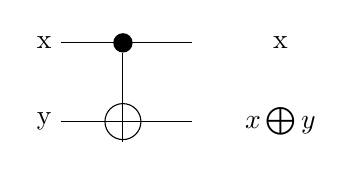
\begin{tikzpicture}
    \tikzstyle{operator} = [draw,shape=circle,fill=white,minimum size=1.3em] 
    \tikzstyle{control} = [fill,shape=circle,minimum size=7pt,inner sep=0pt]
    %
    % Qubits
    \node at (0,0) (x) {\ket{x}};
    \node at (0,-1) (y) {\ket{y}};

    
    % Column 2
    \node[control] (c10) at (1,0) {} ;edge [-] (x);
    \node[operator] (r11) at (1,-1) {} ;edge [-] (y);
    \draw[-] (1,-1.26) -- (c10);

 \node (end1) at (2,0) {} edge [-] (x);
\node (end2) at (2,-1) {} edge [-] (y);

    \node at (3,0) (x) {\ket{x}};
    \node at (3,-1) (y) {$\ket{x} \bigoplus\ket{y}$};

    \end{tikzpicture}
\caption{نمایش دروازه‌ی \lr{CNOT}}
\label{3}
\end{center}
\end{figure}
 همچنین جدول \ref{t1}، جدول درستی این دروازه را نشان می‌دهد.
\begin {table}[h]
\begin{center}
\caption{جدول درستی دروازه‌ي \lr{CNOT}}
\label{t1}
\begin{latin}
 \begin{tabular}{cc|cc}

input&& output&\\
\hline
\ket{x}&\ket{y}&\ket{x}&$\ket{x}\bigoplus \ket{y}$\\
\hline
0&0&0&0\\
\hline
0&1&0&1\\
\hline
1&0&1&1\\
\hline
1&1&1&0\\
\end{tabular}
\end{latin}
\end{center}
\end{table}

\item
دروازه‌های چندکیوبیتی:
در محاسبات کوانتومی تعداد زیادی دروازه‌هایی با بیشتر از دو کیوبیت وجود دارند، اما کاربرد آن‌ها محدود می‌باشد. یکی از پرکاربردترین آن‌ها، دروازه‌ی تافلی\LTRfootnote{\lr{Toffoli}} است. این دروازه دارای دو ورودی کنترلی و یک ورودی هدف است. اگر  \lr{AND} دو کیوبیت هدف بر روی 1 تنظیم شوند، کیوبیت هدف تغییر می‌کند، در غیر اینصورت بدون تغییر می‌ماند. از این دروازه در الگوریتم‌ها و تصحیح خطا کوانتومی استفاده می‌گردد. نمایش ماتریسی و مداری این دروازه در شکل\ref{4} نشان داده شده است. (دو خط بالایی نشان دهنده‌ی کیوبیت کنترلی، خط پایین نشان دهنده کیوبیت هدف است).

\begin{figure}[h]
\begin{center}
\includegraphics{toffoli.jpg}
\caption{نمایش مداری و ماتریسی دروازه \lr{Toffoli}}
\label{4}
\end{center}
\end{figure}

از آن‌جایی که دروازه‌های چند کیوبیت نیاز به دسترسی همزمان به کیوبیت‌ها دارند، پیاده‌سازی آن‌ها دشوار است. به‌طوری که ساخت دروازه‌های تک کیوبیت بسیار آسان، دروازه‌های دو کیوبیتی مقدار کمی پیچیده و ساخت دروازه‌های با بیشتر از دو کیوبیت بسیار پیچیده است. بنابراین می‌توان در یک مدار کوانتومی دروازه‌هایی با بیشتر از دو ورودی حذف شده و آن‌ها را با دروازه های تک‌کیوبیت و دوکیوبیتی جایگزین نمود. از آن‌جایی که در این رساله فقط از دروازه‌های تک‌کیوبیتی و دوکیوبیت استفاده شده است، در صورت مواجه‌شدن با دروازه‌های بیشتر از دو ورودی، آن‌ها با روش‌های سنتز مدارهای کوانتومی جایگزین می‌گردند \cite{marinescu2011classical}. 
%در شکل \ref{5} مدار معادل یک دروازه تافلی با استفاده از دروازه‌های \lr{CNOT} و \lr{V} نشان داده شده است.

%برای مثال شکل \ref{5} یک دروازه \lr{Controlled-U} نشان داده شده است. دروازه‌ی \lr{U} زمانی اعمال می‌شود که هر دو کیوبیت در حالت \ket{1} باشند. در سمت راست، نمایش این دروازه‌ی سه کیوبیتی با استفاده از دو دروازه‌ی \lr{CNOT} و سه دروازه‌ی $V$ و $V^\dag$ به‌طوری‌که $VV^\dag=I$ باشد، پیاده‌سازی شده است.

%\begin{figure}[h]
%\begin{center}
%\includegraphics{toffelitocnot.jpg}
%\caption{مدار معادل یک دروازه‌ی \lr{Controlled-U} و جایگزینی آن با استفاده از دروازه‌های دو کیوبیتی}
%\label{5}
%\end{center}
%\end{figure}
\end{itemize}
\subsection{مدارهای کوانتومی}

ازکنار هم‌قرار‌دادن و اتصال چندین دروازه‌ی کوانتومی، مدارهای کوانتومی\LTRfootnote{\lr{Quantum circuit}} \lr{(QC)} حاصل می‌شوند. هر مدار کوانتومی توسط چندین ویژگی بیان می‌گردد\cite{pham20132d}. این ویژگی‌ها عبارت‌اند‌‌از:
\begin{itemize}
\item
عرض\LTRfootnote{\lr{Width}}مدار \lr{(W)}: بیانگر تعداد کل کیوبیت‌های مورد استفاده در مدار است.
\item
اندازه‌ی\LTRfootnote{\lr{Size}} مدار \lr{(S)}: بیانگر تعداد کل دروازه‌های به‌کار رفته در مدار است.
\item
عمق\LTRfootnote{\lr{Depth}}مدار \lr{(D)}: بیانگر تعداد برش‌های زمانی که جهت اجرای مدار مورد استفاده قرار می‌گیرد. در هر برش زمانی یک یا چند دروازه بسته به ویژگی و محدودیت‌های موجود قابل اجرا هستند.
\end{itemize}
هر مدار کوانتومی از تعدادی خط تشکیل شده است که خطوط از بالا به پایین شماره‌گذاری شده است و تعداد خطوط برابر تعداد کل کیوبیت‌های مورد استفاده در سیستم بوده بطوری که خط $i$ ام بیانگر کیوبیت $q_{i}$ می‌باشد. یک مدار کوانتومی همواره از چپ به راست ارزیابی می‌شود. بنارابن حرکت از چپ به راست در یک مدار کوانتومی به معنای حرکت به جلو در زمان است \cite{khalid2004fpga}.

یکی از کاربردهای مهم محاسبات کوانتومی سنتز مدارهای کوانتومی\LTRfootnote{\lr{Quantum-logic Synthesis}} است. سنتز مدارهاي کوانتومي به فرآيند تبديل يک دروازه‌ي کوانتومي به تعدادي دروازه‌‌ی شناخته شده (با توجه به کتابخانه‌ي دروازه‌هاي جهانی) با قابليت پياده‌سازي در تکنولوژي‌هاي کوانتومي اطلاق مي‌شود. يکي از متداول‌ترين کتابخانه‌هاي دروازه‌های جهانی،  کتابخانه‌ي دروازه‌‌ي پايه\LTRfootnote{\lr{Basic gate library}} است که از دروازه‌ی \lr{CNOT} و کليه‌ي دروازه‌هاي تک کيوبيتي تشکيل شده است. به منظور ارزيابي يک مدار کوانتومي، معيارهاي هزينه مختلفي مانند تعداد دروازه‌های \lr{CNOT} و تک کيوبيتي، هزينه کوانتومی و عمق مدار وجود دارد. پیاده‌سازی مدارهای کوانتومی با استفاده از دروازه‌های جهانی همیشه یک مساله اساسی در محاسبات کوانتومی بوده است. 

از دیگر رایج‌ترین مجموعه‌های جهانی مجموعه‌ی \lr{Clifford+T} است \cite{ross}. این مجموعه شامل دروازه‌های دو کیوبیتی \lr{CNOT}، دروازه‌ي هادامارد و دروازه‌های فاز می‌باشد. هر دروازه‌ی کوانتومی به طور دقیق نمی‌تواند با استفاده از مجموع دروازه‌های جهانی ساخته شود. بلکه با یک تقریب خاصی این کار انجام می‌گردد. بر طبق تئوری \lr{Solovay+Kitaev} که در\cite{dawson2005solovay} ارائه شده است، هر مدار کوانتومی می‌تواند منحصرا با استفاده از هر مجموعه‌ي جهانی از دروازه‌ها در زمان $O(log^{c} \frac{1}{\epsilon})$ با تقریب $\epsilon$ ساخته شود. همچنین سیستم‌های کوانتومی بیشتر از محاسبات کلاسیک در معرض خطا بوده، بنابراین مدارهای کوانتومی تحمل پذیر اشکال برای پیاده‌سازی‌های عملی مورد نیاز هستند. بسیاری از کدهای تصحیح خطای کوانتومی\cite{steane1996error,bacon2006operator,houshmand2012minimal}، جهت ممکن ساختن محاسبات تحمل پذیر اشکال ارائه شده‌اند که تمامی آن‌ها از دروازه‌های جهانی\lr{Clifford+T} استفاده می‌کنند\cite{kliuchnikov2013synthesis}. بنابراین جهت استفاده از این کدها این نیاز وجود دارد تا بتوان هر مدار کوانتومی را با تقریب خاصی توسط مجموعه‌ی جهانی\lr{Clifford+T} ایجاد نمود. 

%از آنجایی‌که این مجموعه‌های جهانی شامل دروازه‌های تک کیوبیتی و دو کیوبیت بوده و دروازه‌های تک کیوبیتی می‌توانند به‌صورت محلی اجرا گردند، جهت توزیع نمودن یک مدار کوانتومی پیاده‌سازی دروازه‌های $CNOT$ به صورت دروازه‌های سراسری کفایت می‌نماید. 


\subsection{پروتکل دورنوردی}
دورنوردی به جابجایی ماده بین دو نقطه بدون پیمودن متداول فضای بین دو نقطه مورد نظر، اشاره می‌کند. به‌عبارت دیگر انتقال یک ماده از یک نقطه به نقطه دیگر بدون عبور از فضای فیزیکی مابین آنهاست. این فناوری شامل تبدیل ماده به نور، انتقال به مقصد و تبدیل مجدد به ماده‌ي اولیه است. تا پیش از کشف کوانتوم، دورنوردی از دیدگاه فیزیک غیرمنطقی انگاشته می‌شد. با این حال سال‌ها طول کشید تا پس از کشف فوتون و خاصیت دوگانه موجی- ذره‌ای نور الکترو‌مغناطیس (اصل دورنوردی)، وجود دورنوردی در ذرات بنیادی به اثبات رسید\cite{furusawa1998unconditional,bouwmeester1997experimental,metcalf2014quantum}.
 این پروتکل یکی از ابزارهای مفید در محاسبات کوانتومی و پردازش اطلاعات آن می‌باشد. زیرا به کمک آن می‌توان کارهایی در مخابرات و اطلاعات کوانتومی انجام داد که بدون آن غیر ممکن است. اين پروتكل طوري است  که بدون اینکه واقعا چیزی به معنی واقعی ارسال شود، می‌تواند یک حالت کوانتومی را به مقصد ارسال نماید. فرض شود آلیس می‌خواهد اطلاعاتی را به دوستش باب ارسال نماید.  آلیس و باب می‌توانند با استفاده از درهم‌تافتگی یک کانال مخابراتی کوانتومی بین خود برقرار نمایند که از طریق جفت \LTRfootnote{\lr{Einstein-Podolsky-Rosen}}\lr{EPR} آن‌ها را به شیوه کوانتومی به‌یکدیگر متصل نماید. به‌عبارتی آلیس می‌تواند اطلاعات خود را به شیوه جادویی به باب ارسال نماید. او تنها می‌تواند بیت‌های کلاسیک و نه بیت‌های کوانتومی را بفرستد. در نگاه نخست، این کار بسیار سخت می‌نماید، چرا که اندازه‌گیری سیستم، حالت آن را به گونه‌ای کنترل ناپذیر آشفته می‌سازد و باب  با این اندازه‌گیری، تنها یک بیت اطلاعات را به دست می‌آورد.

آلیس یک سیستم دو کیوبیتی را در یک حالت نامعلوم در دست دارد و می‌خواهد این کیوبیت را با استفاده از یک کانال مخابراتی به سمت باب بفرستد.

  شکل\ref{8} مدار این پروتکل را نشان می‌دهد.

\begin{figure}[ht]
\begin{center}
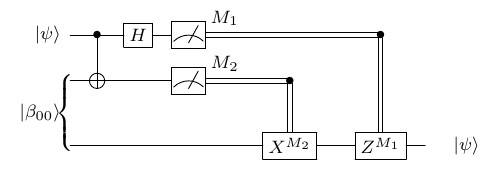
\includegraphics[scale=0.8]{fig8.jpg}
\caption{پروتکل دورنوردی}
\label{8}
\end{center}
\end{figure}
در این مدار دو کیوبیت اول دست آلیس و  کیوبیت سوم دست باب می‌باشد. آلیس قصد دارد حالت کوانتومی خود را باب ارسال نماید. این پروتکل شامل چندین مرحله است: در ابتدا با درست کردن یک زوج در هم تافته \lr{EPR} شروع می‌کنیم.
\begin{itemize}
\item
\textbf{گام اول:}
آلیس و باب یک ذره در‌هم‌تافته بوجود می‌آورند. این حالت در رابطه \eqref{eq10} نشان داده شده است. در این رابطه فرض شده است که اولین کیوبیت متعلق به آلیس و دومین آن متعلق به باب باشد. آلیس و باب به لحاظ فیزیکی فاصله‌ی دوری از هم دارند.
\begin {equation}
\ket{\beta_{00}}=\frac{\ket{0_{A}}\ket{0_{B}}+\ket{1_{A}}\ket{1_{B}}}{\sqrt{2}}=\frac{\ket{00}+\ket{11}}{\sqrt{2}}
\label{eq10}
\end{equation}
\item
\textbf{گام دوم: }
حالت کل سیستم به صورت ضرب تانسوری سه کیوبیت به صورت رابطه‌ي \eqref{eqt} می‌باشد:
\begin{equation}
\ket{\psi}=\ket{\chi}\oplus \ket{\beta_{00}}=(\alpha\ket{0}+\beta\ket{1})\otimes(\frac{\ket{00}+\ket{11}}{\sqrt{2}})
 =\frac{\alpha \ket{000}+\ket{011}+\beta(\ket{100}+\ket{111})}{\sqrt{2}}
\label{eqt}
\end{equation}


دوکیوبیت اول در این حالت متعلق به آلیس است و سومین کیوبیت (سمت راست‌ترین) متعلق به باب است. بنابراین حالت کوانتومی \ket{011} بیان‌گر این است که آلیس 01 دارد و باب 1. سپس آلیس با اعمال یک دروازه \lr{CNOT} امکان می‌دهد که بیت‌های خودش در زوج \lr{EPR} که کیوبیت دوم در معادله بالا است، با حالت ناشناخته که اولین کیوبیت در معادله بالاست، برهم کنش داشته باشد. از حالت ناشناخته \ket{\psi} به عنوان بیت کنترل استفاده می‌کند و نتیجه ارائه شده در رابطه‌ی \eqref{eqtt} حاصل می‌شود.
\begin{equation}
\begin{split}
 \ket{\psi^{'}}=U_{CNOT}\ket{\psi} \\
=\frac{\alpha(U_{CNOT}\ket{000}+U_{CNOT}\ket{011})+\beta(U_{CNOT}\ket{100}+U_{CNOT}\ket{111})}{\sqrt{2}} \\
 =\frac{\alpha \ket{000}+\ket{011}+\beta(\ket{110}+\ket{101})}{\sqrt{2}}
\end{split}
\label{eqtt}
\end{equation}
\item
\textbf{ گام سوم: }
در این مرحله آلیس یک دروازه‌ی هادامارد به کیوبیت اول اعمال می‌کند. حالت جدید سیستم پس از اعمال این دروازه به صورت رابطه‌ی \eqref{eq13} محاسبه می‌گردد.
\begin{equation}
\begin{split}
 \ket{\psi^{''}}=H\ket{\psi^{'}}=\frac{\alpha H\ket{0}(\ket{00}+\ket{11})+\beta H\ket{1}(\ket{10}+\ket{01})}{\sqrt{2}} \\
 =\alpha(\frac{\ket{0}+\ket{1}}{\sqrt{2}})\frac{(\ket{00}+\ket{11})}{\sqrt{2}}+\beta(\frac{\ket{0}-\ket{1}}{\sqrt{2}})\frac{(\ket{10}+\ket{01})}{\sqrt{2}}
\end{split}
\label{eq13}
\end{equation}
دقت شود کیوبیت سوم دست باب می‌باشد.

\item
\textbf{گام چهارم:}
در این مرحله آلیس دو کیوبیت در دست خود را اندازه گیری می‌نماید. حالت‌هاي مختلفی که از نتایج اندازه گیری بدست می‌آید، در رابطه‌ی \eqref{eq14} نوشته شده است:

\begin{equation}
\begin{split}
\ket{\psi^{''}}=\frac{1}{2}(\ket{00}(\alpha\ket{0}+\beta\ket{1})+\ket{01}(\alpha\ket{1}+\beta\ket{0})+\ket{10}(\alpha\ket{0}-\beta \ket{1})+\ket{11}(\alpha\ket{1}-\beta\ket{0}))
\end{split}
\label{eq14}
\end{equation}

معادله‌ی \eqref{eq14} بیان می‌کند چنانجه آلیس \ket{00} را اندازه‌گیری نماید$ \ket{\chi}=\alpha\ket{0}+ \beta\ket{1}$ را خواهد داشت، یعنی همان حالت ناشناخته‌ای که آلیس خواسته تا به باب ارسال نماید. حال اگر آلیس حالت \ket{01} را اندازه گیری نماید، آنگاه باب حالت
   $\alpha\ket{1}+ \beta\ket{0}$
را در دست دارد. ولی می‌تواند با اعمال دروازه‌ی \lr{X}  آن را به حالت دلخواه خود تبدیل نماید.
چنانچه آلیس حالت \ket{01} را اندازه گیری نماید، باب حالت $\alpha\ket{0}-\beta\ket{1}$  را داراست که می‌توان با اعمال دروازه \lr{Z} آن را به حالت دلخواه خود تبدیل نماید.

در نهایت چنانچه آلیس حالت $\ket{11}$  را اندازه بگیرد، باب حالت$\alpha\ket{1}-\beta\ket{0}$ را داراست. و این بار باب باید دو دروازه\lr{X} و \lr{Z} را پشت سرهم اعمال نماید تا حالت$\ket{\psi}$  بدست بیاد.

\item
\textbf{گام پنجم:}
در مرحله‌ی چهارم برای اطلاع ازینکه باب از کجا بداند چه دروازه‌ای را اعمال نماید، بایستی یک کانال مخابراتی کلاسیک مانند تلفن، موج رادیویی یا ایمیل انجام دهد.

\end{itemize}

\section{سیستم‌های کوانتومی توزیع شده}
 یکی از محدودیت‌های پیاده‌سازی مدارهای کوانتومی، این است که با افزایش تعداد کیوبیت‌ها، اطلاعات کوانتومی با خطا مواجه می‌شوند.  همچنین معماری محاسبات کوانتومی قادر به اجرای چنین مدارهای بزرگی نمی‌باشد\cite{Pablo}. برای غلبه بر این مشکل، می‌توان مدار کوانتومی را در چند زير سيستم كوانتومي توزيع نمود به‌طوری که هر سيستم روي یک واحد پردازنده کوانتومی مجزا به‌نام \lr{(QPU)}\LTRfootnote{\lr{Quantum Processing Unit}} اجرا گردد. این راه حل منجر به یک مصالحه می‌گردد: هرچه تعداد زیر مدارها یا واحدها بیشتر گردد، هزینه‌ی محاسباتی بیشتر خواهد شد. برای داشتن یک سیستم کوانتومی در مقیاس بزرگ بهتر آن است تا شبکه‌ای از سیستم‌های کوانتومی دارای ظرفیت محدود به لحاظ تعداد کیوبیت‌ها در نظر گرفته شود.
 
 سیستم‌های کوانتومی توزیع شده شامل مجموعه‌ای از کامپیوترهای کوانتومی مستقل \LTRfootnote{\lr{Independent}} است، که برای کاربر خود مانند یک سیستم منسجم و منفرد به نظر برسد. هر یک از این سیستم‌ها می‌تواند از لحاظ سخت‌افزاری و یا نرم‌افزاری با یکدیگر متفاوت باشد. همچنین در سیستم‌های کوانتومی برای جلوگیری و محافظت از اطلاعات کوانتومی از نویز و ناهمدوسی کیوبیت‌ها، هر سیستم دارای توپولوژی ارتباطی و محدودیت‌های فیزیکی خاص بین کیوبیت‌هایش می‌باشد. این محدودیت‌های فیزیکی بایستی از دید کاربر سیستم‌ کوانتومی توزیع شده (الگوریتم کوانتومی) مخفی بماند.
\subsection{معماری سیستم‌های کوانتومی توزیع شده}
شکل \ref{ar} معماری یک سیستم کوانتومی توزیع شده را نشان می‌دهد. الگوریتم کوانتومی در قالب مدار کوانتومی در بالاترین سطح به عنوان ورودی سیستم در نظر گرفته می‌شود. و هدف آن اجرای یک وظیفه‌ی کاربر با استفاده از محاسبات کوانتومی است. مدار کوانتومی داده شده در بالاترین سطح، برحسب تعداد ورودی‌ها مانند تعداد کیوبیت‌ها و عمق مدار از طریق لایه‌ی سیستم کوانتومی توزیعی بین سیستم‌های کوانتومی توزیع می‌گردد. در واقع نقش توزیع نمودن مدار به طور کارا مابین سیستم‌های کوانتومی از وظایف لایه سیستم کوانتومی توزیعی است. سپس با توزیع مناسب کیوبیت‌ها در بین سیستم‌های کوانتومی و در نظر توپولوژی‌های فیزیکی هر زیر سیستم، حالت‌هاي کوانتومی به سیستم های کوانتومی داده شده و آن‌ها با تعدادی عملگرهای محلی و سراسری مواجه می‌گردند. عملگرهای محلی به طور محلی در هر زیر سیستم اعمال می‌شوند. اما عملگرهای سراسری  برای اجرای خود نیاز به کیوبیت‌های سایر سیستم ها دارند. سیستم‌های کوانتومی برای ارتباط با سایر سیستم‌های کوانتومی نیاز به سخت افزار تولید زوج‌های درهم تنیده دارند \cite{Pablo} تا حالت‌هاي کوانتومی را بین خود به اشتراک بگذارند. بنابراین در پایین لایه نیاز به یک سخت افزار جهت تولید این زوج‌ها می‌باشد. علاوه بر لینک‌های کوانتومی بین سیستم‌ها، نیاز به یک کانال ارتباطی کلاسیک نیز بوده، تا کیوبیت‌ها بتواند پس از اندازه‌گیری حالت‌هاي خود، اطلاعات خود ار ازطریق سیستم کلاسیک به سایر سیستم‌ها ارسال نمایند. 

\begin{figure}[h]
\begin{center}
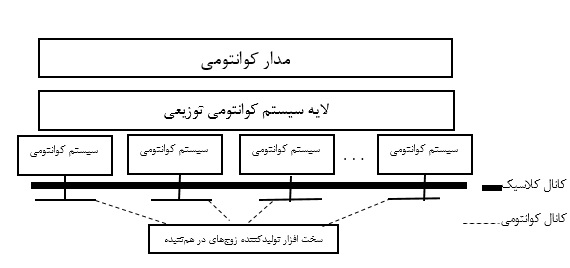
\includegraphics[scale=0.8]{architect.jpg}
\caption{معماری سیستم کوانتومی توزیع شده}
\label{ar}
\end{center}
\end{figure}
همان‌طور که در سیستم‌های توزیع شده کلاسیک، اهداف و ویژگی‌های مشخصی وجود دارد \cite{tanenbaum2007distributed}، در سیستم‌های کوانتومی توزیع شده نیز می‌توان این اهداف و ویژگی‌ها را برشمرد. اهدافی که در طراحی یک سیستم کوانتومی توزیع شده مد نظر قرار می‌گیرند، عبارت‌اند از:
\begin{itemize}
\item
دسترس‌پذیری\LTRfootnote{\lr{Accessibility}}: هدف اصلی سیستم کوانتومی توزیع شده این است تا کاربران (برنامه‌های کاربردی) بتوانند به راحتی به سایر سیستم‌های کوانتومی دسترسی پیدا کرده و محاسبات خود را انجام دهند. برای مثال با توجه به این‌که تعداد کیوبیت‌هایی که یک سیستم کوانتومی می‌تواند پردازش نماید، محدود است، بایستی بتوان سیستمی طراحی نمود تا امکان استفاده ازکیوبیت‌های سایر سیستم‌ها فراهم گردد.
\item
مخفی‌سازی\LTRfootnote{\lr{Transparency}}: بایستی سیستم توزیع شده بتواند به لحاظ دسترسی\LTRfootnote{\lr{Access}}، مکان \LTRfootnote{\lr{Location}}، مهاجرت\LTRfootnote{\lr{Migration}} و جابجایی\LTRfootnote{\lr{Relocation}} شفاف‌سازی شود. برای مثال شفاف‌سازی در دسترسی به سایر سیستم‌ها به این معناست که الگوریتم کوانتومی (کاربر) تصور کند که از لحاظ دسترسی، تمامی سیستم‌ها در یک مکان قرار دارند. به‌عبارتی بعد فاصله از دید آن مخفی باشد. همان‌طور که قبلا بیان گردید، با استفاده از پروتکل دورنوردی می‌توان اطلاعات کوانتومی را در فواصل زیاد بدون پیمایش فاصله فیزیکی بین آن‍ها جابجا و منتقل نمود، بنابراین با این قاعده می‌توان گفت هر چهار شفافیت بیان شده که در سیستم‌های توزیع شده کلاسیک \cite{tanenbaum2007distributed} وجود دارد، می‌تواند در سیستم‌های کوانتومی توزیع شده نیز وجود داشته باشد. اما برای مثال شفافیت‌سازی تکثیر \LTRfootnote{\lr{Replication Transparency}} که یکی از ویژگی‌ها و اهداف سیستم‌های توزیع شده‌ی کلاسیک می‌باشد، در مبحث سیستم‌های کوانتومی توزیع شده با سختی امکان‌پذیر است. زیرا در شفاف‌سازی تکثیر ممکن است درخواست‌ها برای منبع زیاد باشد و نیاز باشد از یک منبع یا اطلاعات کوانتومی چندین تکثیر انجام شود. اما بر طبق تئوری عدم تکثیر کوانتومی، نمی‌توان تکثیری از حالت‌هاي کوانتومی داشت. بنابراین تکثیر و شفاف سازی آن در مبحث سیستم‌های کوانتومی توزیع شده با مشکل مواجه می‌گردد و نیاز به استفاده از هزینه‌ی دورنوردی و همگام‌سازی اطلاعات کوانتومی است.
\item
باز بودن سیستم\LTRfootnote{\lr{Openness}}: این ویژگی از سیستم‌های کوانتومی توزیع شده به این معناست که به راحتی بتوان به سیستم توزیع شده متصل شد و سرویس گرفت و یا سرویسی را از آن به راحتی جدا نمود.

\item
گسترش‌پذیری\LTRfootnote{\lr{Scalibility}}: یکی از اهداف اصلی در سیستم‌های کوانتومی توزیع شده، توسعه پذیری یا گسترش‌پذیری آن است. مفهوم توسعه پذیری در سیستم‌های کوانتومی توزیع شده را به این صورت می‌توان مطرح کرد. اگر در بالاترین لایه، الگوریتم کوانتومی شامل تعداد زیادی کیوبیت در ورودی خود باشد، بایستی سیستم مقیاس‌پذیر بوده و بتواند جهت انجام الگوریتم کوانتومی با تعداد کیوبیت بالا بدون مشکل پاسخ‌گو باشد. برای این کار دو راهکار وجود دارد: تعداد سیستم‌های کوانتومی را افزایش داد \lr{(Scale up)} و یا اینکه کیوبیت‌های هر سیستم کوانتومی را افزایش داد \lr{(Scale in)}. راه حل دوم با مشکل افزایش تعداد کیوبیت‌های سیستم در هر زیر سیستم مواجه است. اما ‌می‌توان تعداد سیستم‌های کوانتومی را افزایش داد که با افزایش هزینه مواجه می‌شویم. زیرا ارتباط‌ها سراسری و تعداد استفاده از پروتکل دورنوردی افزایش یافته و در نتیجه کارایی سیستم کاهش می‌یابد. 
\end{itemize}





\section{ اصطلاحات مورد استفاده در سیستم‌های کوانتومی توزیع شده}
\subsection{افراز}
از آنجایی که سیستم‌های کوانتومی از تعدادی زیر سیستم کوانتومی تشکیل شده و هدف توزیع کیوبیت‌‌ها بین این سیستم‌های کوانتومی است، با یک مساله افرازبندی\LTRfootnote{\lr{Partitioning}} مواجه هستیم. بنابراین منظور از افراز در این رساله، همان زیر سیستم‌های کوانتومی می‌باشد.
 

\subsection{دروازه‌های محلی و سراسری}
در سیستم‌های کوانتومی توزیع شده، با افرازبندی و توزیع کیوبیت‌ها در تعدادی سیستم کوانتومی، دروازه‌های مدار به دو دسته‌ی دروازه‌های محلی و دروازه‌های سراسری تقسیم می‌شوند که در ادامه به بیان هر یک از آن‌ها پرداخته شده است.
\begin{itemize}
\item
\textbf{دروازه‌های محلی:}

در این دروازه‌ها، کیوبیت‌های مورد نیاز جهت اجرای آن‌ها، در یک سیستم کوانتومی قرار داشته و دورنوردی کوانتومی مورد نیاز نمی‌باشد.

از آنجایی‌که مجموعه‌ی کتابخانه‌ی مورد استفاده در این رساله، کتابخانه‌ی پایه بوده و این کتابخانه شامل دروازه‌ی دوکیوبیتی \lr{CNOT} و تک کیوبیتی‌ها است، دروازه‌های محلی می‌تواند شامل دروازه‌های تک کیوبیتی و دو کیوبیتی باشد که به صورت زیر در این رساله نشان داده می‌شود:


دروازه‌ی تک کیوبیتی: در این رساله دروازه‌ی تک کیوبیتی به‌صورت فرمول \eqref{eq23} نشان داده خواهد شد.
\begin{equation}
g(q_{i},P_{i})
\label{eq23}
\end{equation}
بطوری که $q_{i}$ بیانگر شماره کیوبیتی است که دروازه‌ی تک کیوبیتی روی آن عمل نموده و $P_{i}$ بیانگر شماره افرازی است که کیوبیت $q_{i}$ در آن قرار دارد.



دروازه‌ی دو کیوبیتی: دروازه‌های دو کیوبیتی و محلی به صورت فرمول \eqref{eq24} نشان داده می‌شوند.
\begin{equation}
CNOT(q_{t},q_{c},P_{t})
\label{eq24}
\end{equation}
عبارت بالا بیانگر این است که این دروازه‌ی محلی دارای کیوبیت کنترلی $q_{t}$ و کیوبیت هدف $q_{c}$ بوده و این کیوبیت‌ها در یک افراز به نام $P_{t}$ قرار دارند. 

\item
\textbf{دروازه‌های سراسری:}

در این دروازه‌ها، کیوبیت‌های مورد نیاز برای اجرای آن‌ها، در سیستم‌های کوانتومی مجزا قرار داشته و نیاز است که آن‌ها با استفاده از پروتکل دورنوردی در یک سیستم قرار بگیرند.



\begin{equation}
CNOT(q_{c},q_{t},P_{c},P_{t})
\label{eq25}
\end{equation}

عبارت بالا بیان می‌کند که دروازه‌ی \lr{CNOT} به ترتیب دارای کیوبیت هدف و کنترلی $q_{t}$ و $q_{c}$ بوده که به‌ترتیب در افراز‌های $P_{t}$ و $P_{c}$ قرار دارند.
\end{itemize}
در ادامه در ابتدا به بیان نمادها و تعاریف مورد استفاده، سپس به توضیح و پیاده‌سازی روش‌های پیشنهادی پرداخته شده است.


برای مثال، مدار ارائه شده در شکل \ref{13} در دو افراز \lr{$P_{1}$} و \lr{$P_{2}$} توزیع شده است. در این افرازبندی، دروازه‌های \lr{$g_{1},g_{4},g_{5},g_{7}$}  دروازه‌های محلی و دروازه‌های \lr{$g_{2},g_{3},g_{6}$} دروازه‌های سراسری محسوب می‌گردند.
\begin{figure}[ht]
\begin{center}   \begin{tikzpicture}
    \node at (0,0) (q1) {\ket{q_{1}}};
    \node at (0,-1) (q2) {\ket{q_{2}}};
    \node at (0,-2) (q3) {\ket{q_{3}}};
    \node at (0,-3) (q4) {\ket{q_{4}}};

    
    % Column 2
    \node[control] (c20) at (2,0) {} ;edge [-] (q1);
    \node[operator] (r21) at (2,-1) {} ;edge [-] (q2);
    \draw[-] (2,-1.3) -- (c20);

 % Column 3
    \node[control] (c31) at (3,-1) {}; %edge [-] (q2);
    \node[operator] (r33) at (3,-2) {}; %edge [-] (q3);
   \draw[-] (c31) -- (3,-2.3);

 % Column 4
    \node[control] (r40) at (4,0) {} ;%edge [-] (r32);
    \node[operator] (c42) at (4,-2) {};% edge [-] (q2);
    \draw[-] (4,-2.3) -- (r40);
    %
   % Column 5
    \node[operator] (r52) at (5,-2) {} ;%edge [-] (r32);
    \node[control] (c53) at (5,-3) {};% edge [-] (q2);
    \draw[-] (5,-1.7) -- (c53);
    %
   
% Column 6
    \node[control] (r62) at (6,-2) {} ;%edge [-] (r32);
    \node[operator] (c63) at (6,-3) {};% edge [-] (q2);
    \draw[-] (6,-3.3) -- (r62);

%Column 7
 \node[control] (r71) at (7,-1) {} ;%edge [-] (r32);
    \node[operator] (c72) at (7,-2) {};% edge [-] (q2);
    \draw[-] (7,-2.3) -- (r71);

%Column 8
 \node[control] (r82) at (8,-2) {} ;%edge [-] (r32);
    \node[operator] (c83) at (8,-3) {};% edge [-] (q2);
    \draw[-] (8,-3.3) -- (r82);

 \node (end1) at (9,0) {} edge [-] (q1);
\node (end2) at (9,-1) {} edge [-] (q2);
 \node (end3) at (9,-2) {} edge [-] (q3);
 \node (end4) at (9,-3) {} edge [-] (q4);

%part
\draw [line1,dashed](-1,-1.5)-- (9.5,-1.5);
%\draw  [line1,dashed](-1,-1.5)-- (9.5,-1.5);
 \node at (-1,0)  {$P_{1}$};  \node at (-1,-2) {$P_{2}$}; %\node at (-1,-2)  {$p_{3}$};
%gate
\draw [line2,dashed](2.5,0.5)-- (2.5,-4);
\draw  [line2,dashed](3.5,0.5)-- (3.5,-4);
\draw  [line2,dashed](4.5,0.5)-- (4.5,-4);
\draw  [line2,dashed](5.5,0.5)-- (5.5,-4);
\draw  [line2,dashed](6.5,0.5)-- (6.5,-4);
\draw  [line2,dashed](7.5,0.5)-- (7.5,-4);
  \node at (2,-4)  {$g_{1}$};  \node at (3,-4)  {$g_{2}$};  \node at (4,-4)  {$g_{3}$};  \node at (5,-4)  {$g_{4}$}; 
 \node at (6,-4)  {$g_{5}$};  \node at (7,-4)  {$g_{6}$};   \node at (8,-4)  {$g_{7}$}; 
    \end{tikzpicture}
\caption{مثالی از یک مدار توزیع شده در دو افراز $P_{1}$ و $P_{2}$}
\label{13}
\end{center}
\end{figure}
\section{خلاصه}

در این فصل، مروری بر مفاهیم اولیه مورد نیاز در زمینه محاسبات کوانتومی و محاسبات کوانتومی توزیع شده برای درک بهتر ادامه‌ی این رساله ارائه شد. همچنین معماری لایه‌ای سیستم‌های کوانتومی توزیع شده ارائه  گردید. در ادامه در فصل آینده، کارهای پیشین و مرتبط به این رساله مطرح خواهند شد.
